\section{Obtención de velocidad}

Como se menciono anteriormente en la Sección \ref{cap:metodologia} la obtención de la velocidad se divide en tres partes las cuales están representadas en el Figura \ref{fig:DFObtencionDeVelocidad} y se describen a lo largo de esta sección.

\begin{figure}[H]
    \centering
    \begin{tikzpicture}

        \node(a0)[rectangle,
            draw=black,
            minimum width=7cm,
            minimum height=5.7cm,
            label=Obtención de velocidad]
            {};

        \node(a)[rectangle, draw=black, minimum width=5cm, minimum height=1cm] at ([yshift=-2em]a0.north)
        % [inside=of a0]
            {Extracción  de caracteristicas};

        \node(b)[rectangle, draw=black, minimum width=5cm, minimum height=1cm]
            [below=of a]
            {Modelo predictivo};

        \node(c)[rectangle, draw=black, minimum width=5cm, minimum height=1cm]
            [below=of b]
            {Obtención de la velocidad};

        \draw[->] (a) -- (b);
        \draw[->] (b) -- (c);

    \end{tikzpicture}

    \caption{Proceso de obtención de velocidad.}
    \label{fig:DFObtencionDeVelocidad}
\end{figure}

\subsection{Extracción de caracteristicas }

Una vez que hemos tomado la muestra y generado el archivo CSV relacionado podemos ejecutar el sistema para extraer las características que nos interesa junto a la velocidad detectada por el radar de velocidad.

El sistema se encarga de leer el video utilizando la biblioteca OpenCV con la cual examina fotograma por fotograma, e identifica los vehículos utilizando la red neuronal YOLO, una vez que tiene identificados todos los vehículos dibuja la caja correspondiente a cada uno de ellos. La Figura \ref{fig:LugarDeteccion} muestra 2 vehículos detectados, los cuales están dentro de un recuadro.

\begin{figure}[H]
    \centering
    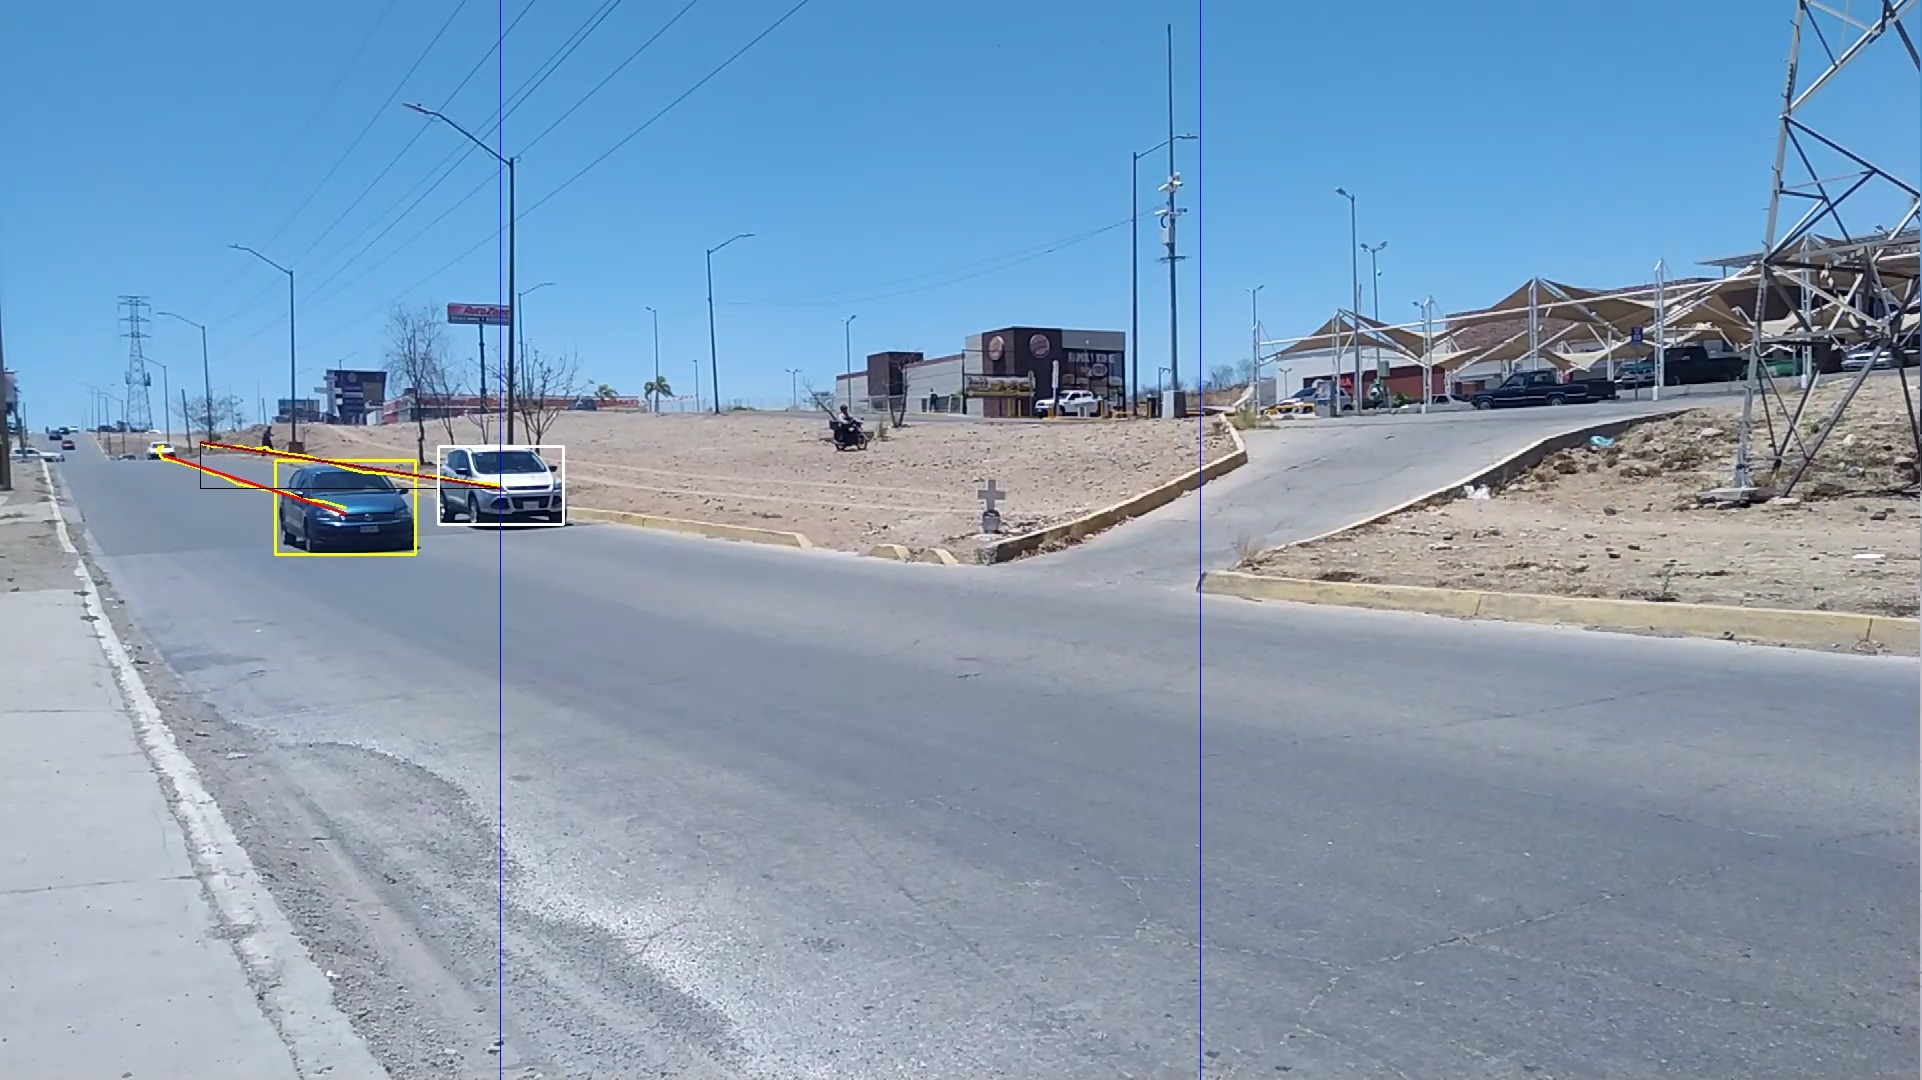
\includegraphics[width=0.8\textwidth]{Metodologia/imgs/Deteccion.jpg}
    \caption{Detección de vehículos dentro de recuadros.}
    \label{fig:LugarDeteccion}
\end{figure}

El seguimiento de los vehículos se realiza por medio del Filtro Kalman para determinar su ubicación en el próximo fotograma. El sistema se encarga de guardar todas las ubicaciones de los vehículos en el transcurso del tiempo, con lo cual es capaz dibujar todo el trayecto que han tenido cada uno de ellos y con el uso de regresión lineal podemos generar una recta que corresponde a las trayectorias de los vehículos, la Figura \ref{fig:LugarSeguimiento} muestra un vehículo detectado en un recuadro blanco, así como un par de líneas una amarilla y otra roja que corresponden al seguimiento del mismo y a la recta calculada correspondiente al seguimiento.

\begin{figure}[H]
    \centering
    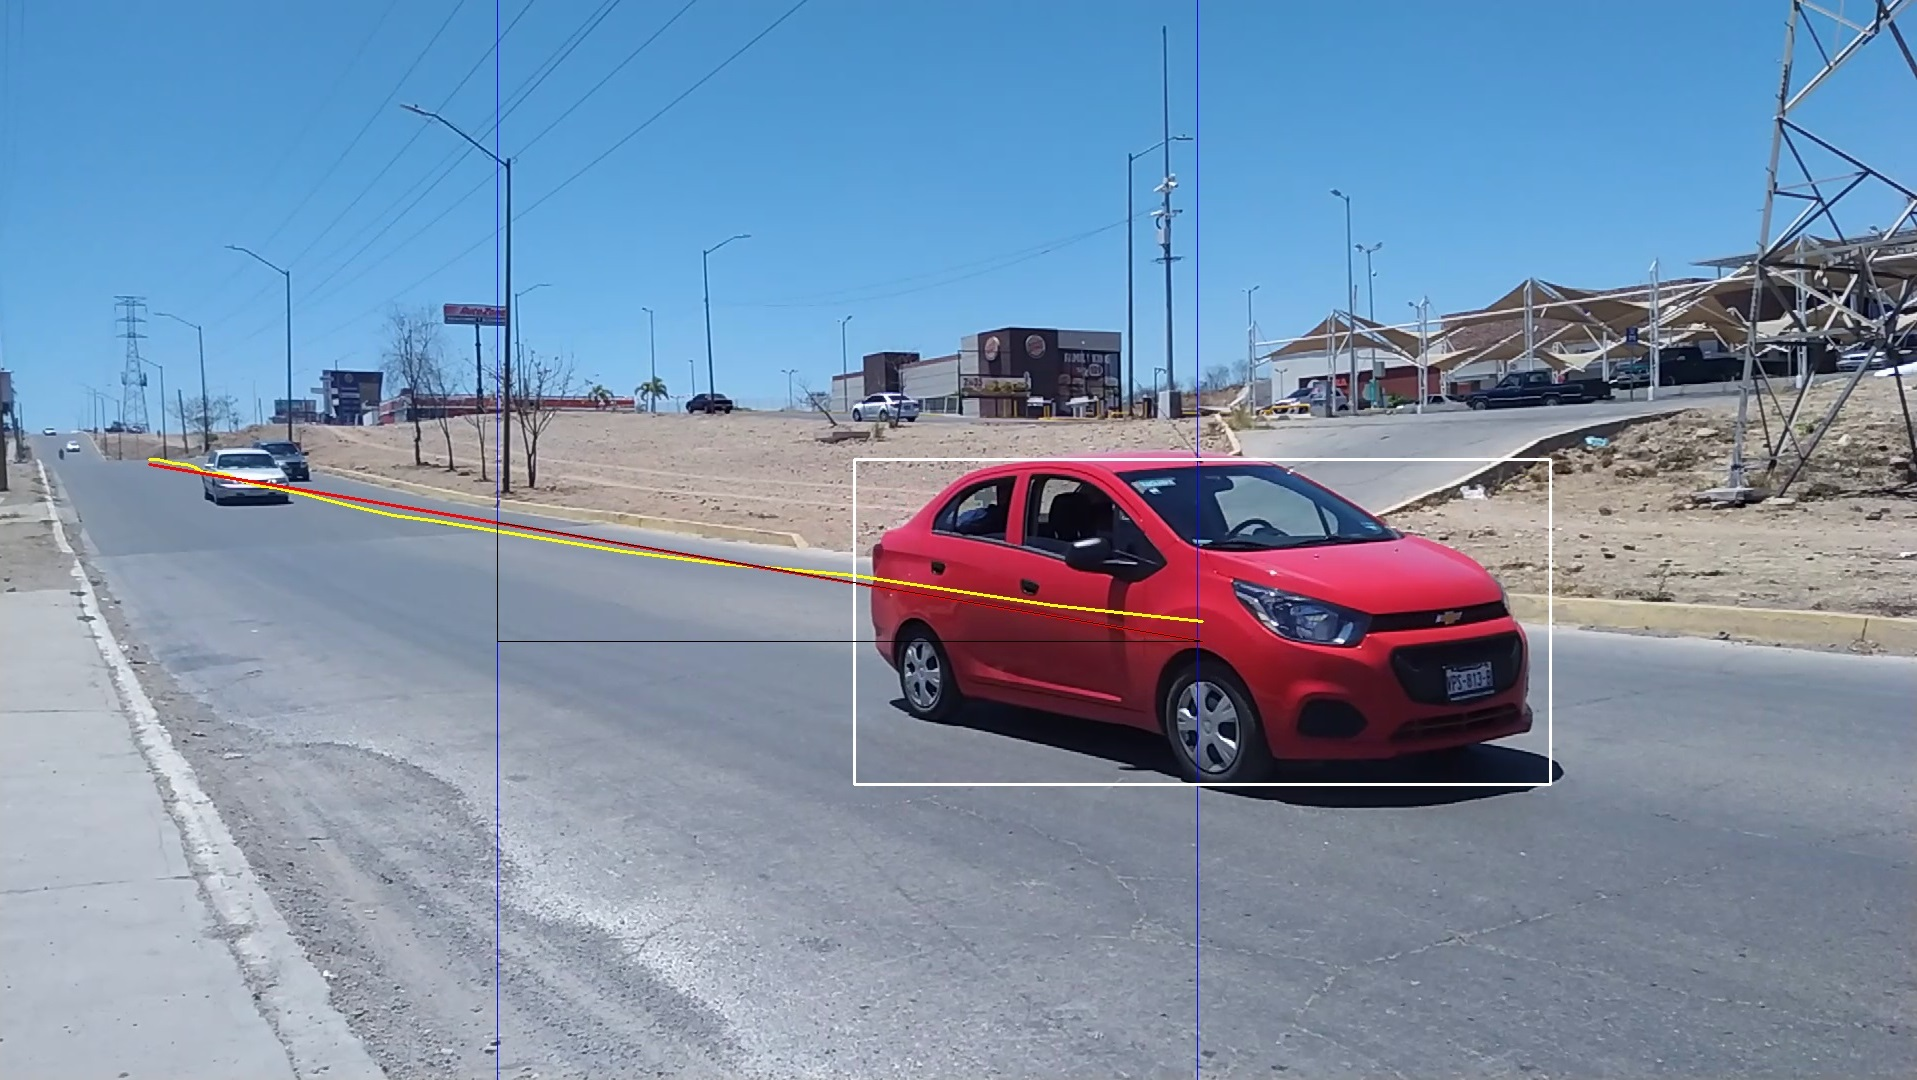
\includegraphics[width=0.8\textwidth]{Metodologia/imgs/Seguimiento.jpg}
    \caption{Detección de vehículos y sus trayectorias.}
    \label{fig:LugarSeguimiento}
\end{figure}

Otra característica que podemos identificar en la Figura \ref{fig:LugarSeguimiento} es la creación de un triángulo en color negro, con el cual podemos identificar el ángulo detectado para el vehículo.

Cando el sistema detecta que un vehículo pasa por el punto A, este guarda la información del estado del vehículo Figura \ref{fig:PuntoA}, puede haber múltiples vehículos pasando en ese momento y todos serán detectados por YOLO, sin embargo, podemos identificar el vehículo del cual se está guardando su estado con el recuadro blanco, ya que para el resto de vehículos se dibuja un recuadro amarillo.

\begin{figure}[H]
    \centering
    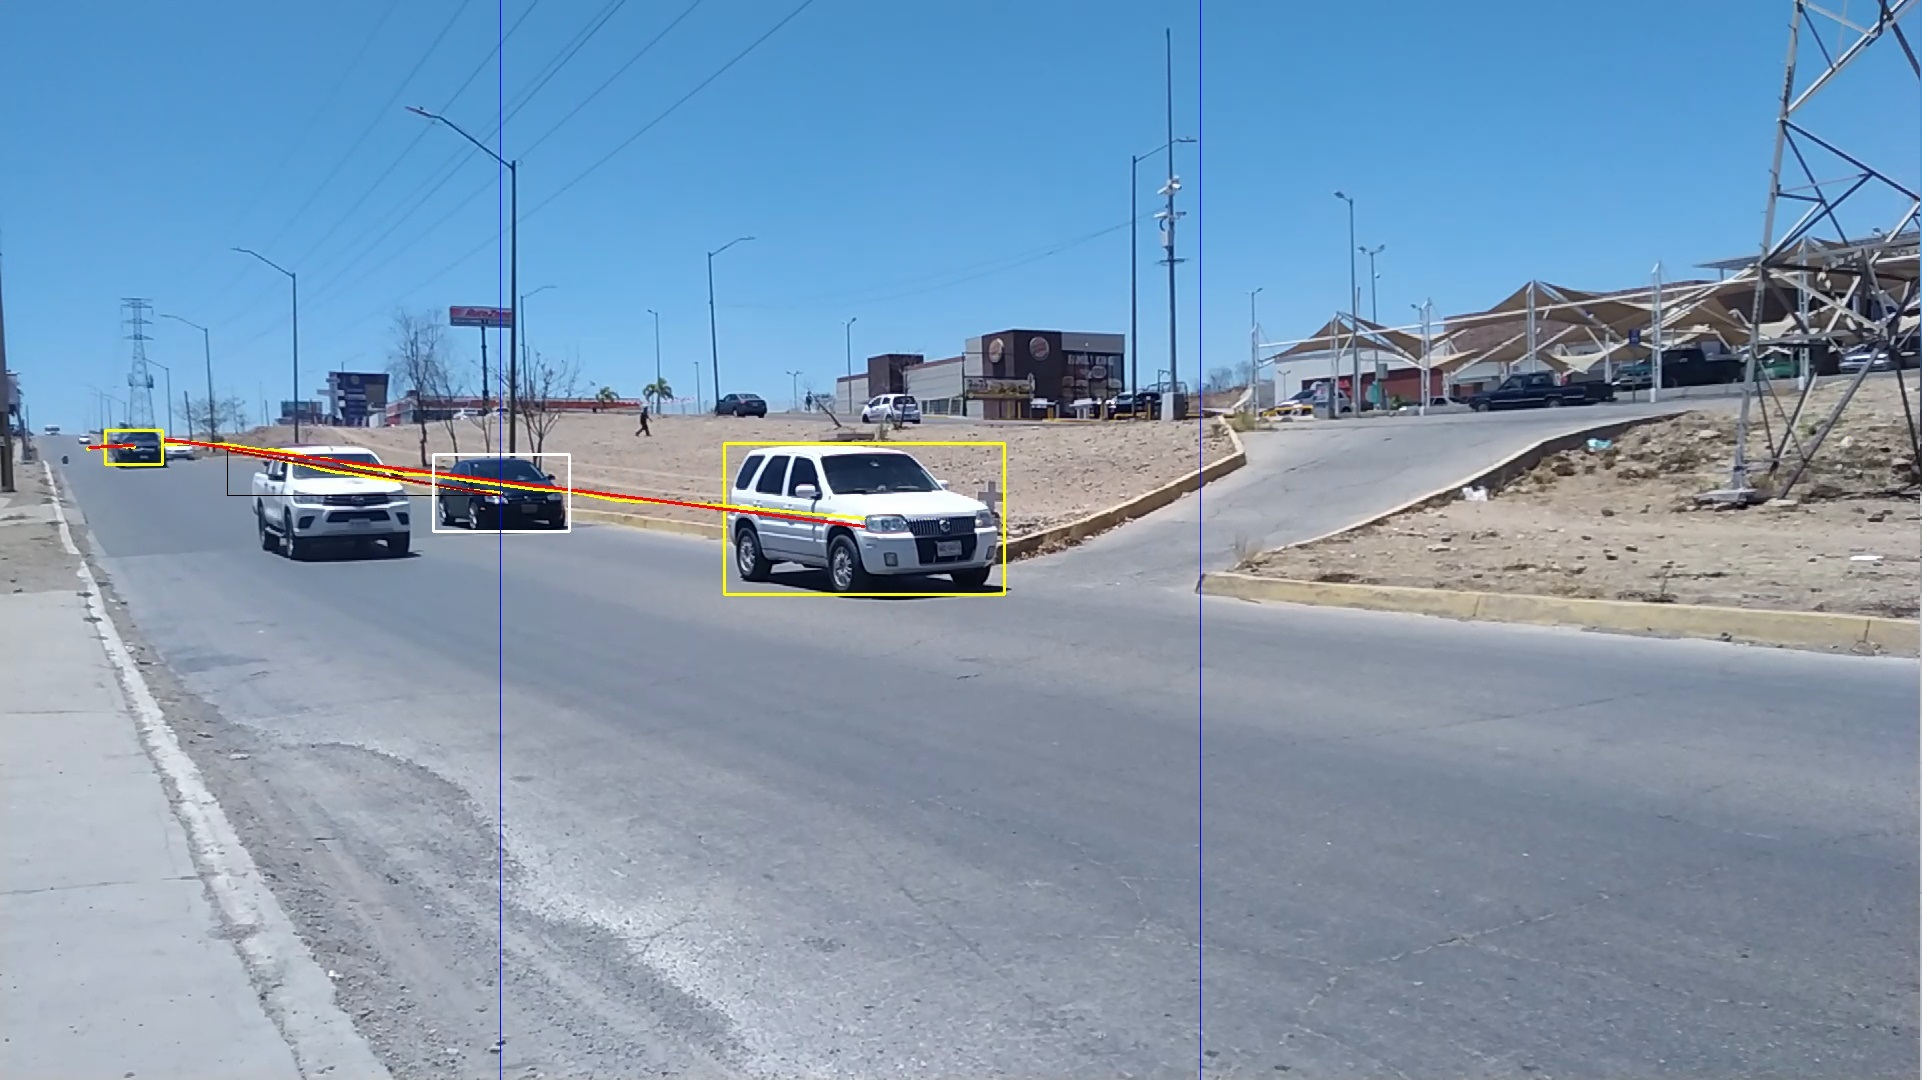
\includegraphics[width=0.8\textwidth]{Metodologia/imgs/Punto_A.jpg}
    \caption{Punto A con vehículo en recuadro blanco.}
    \label{fig:PuntoA}
\end{figure}

Aunque se guardó el estado del vehículo cuando paso por el punto A, este no genera una línea para el archivo CSV resultante, es hasta que el vehículo pasa por el punto B y coincide con los segundos en el archivo CSV de entrada que el sistema guarda un nuevo dato en el archivo de salida, los vehículos que no cuentan con una línea en el archivo CSV de entrada no se les guarda su información. La Figura \ref{fig:PuntoB} muestra cuando el vehículo detectado en el punto A pasa por el punto B.

\begin{figure}[H]
    \centering
    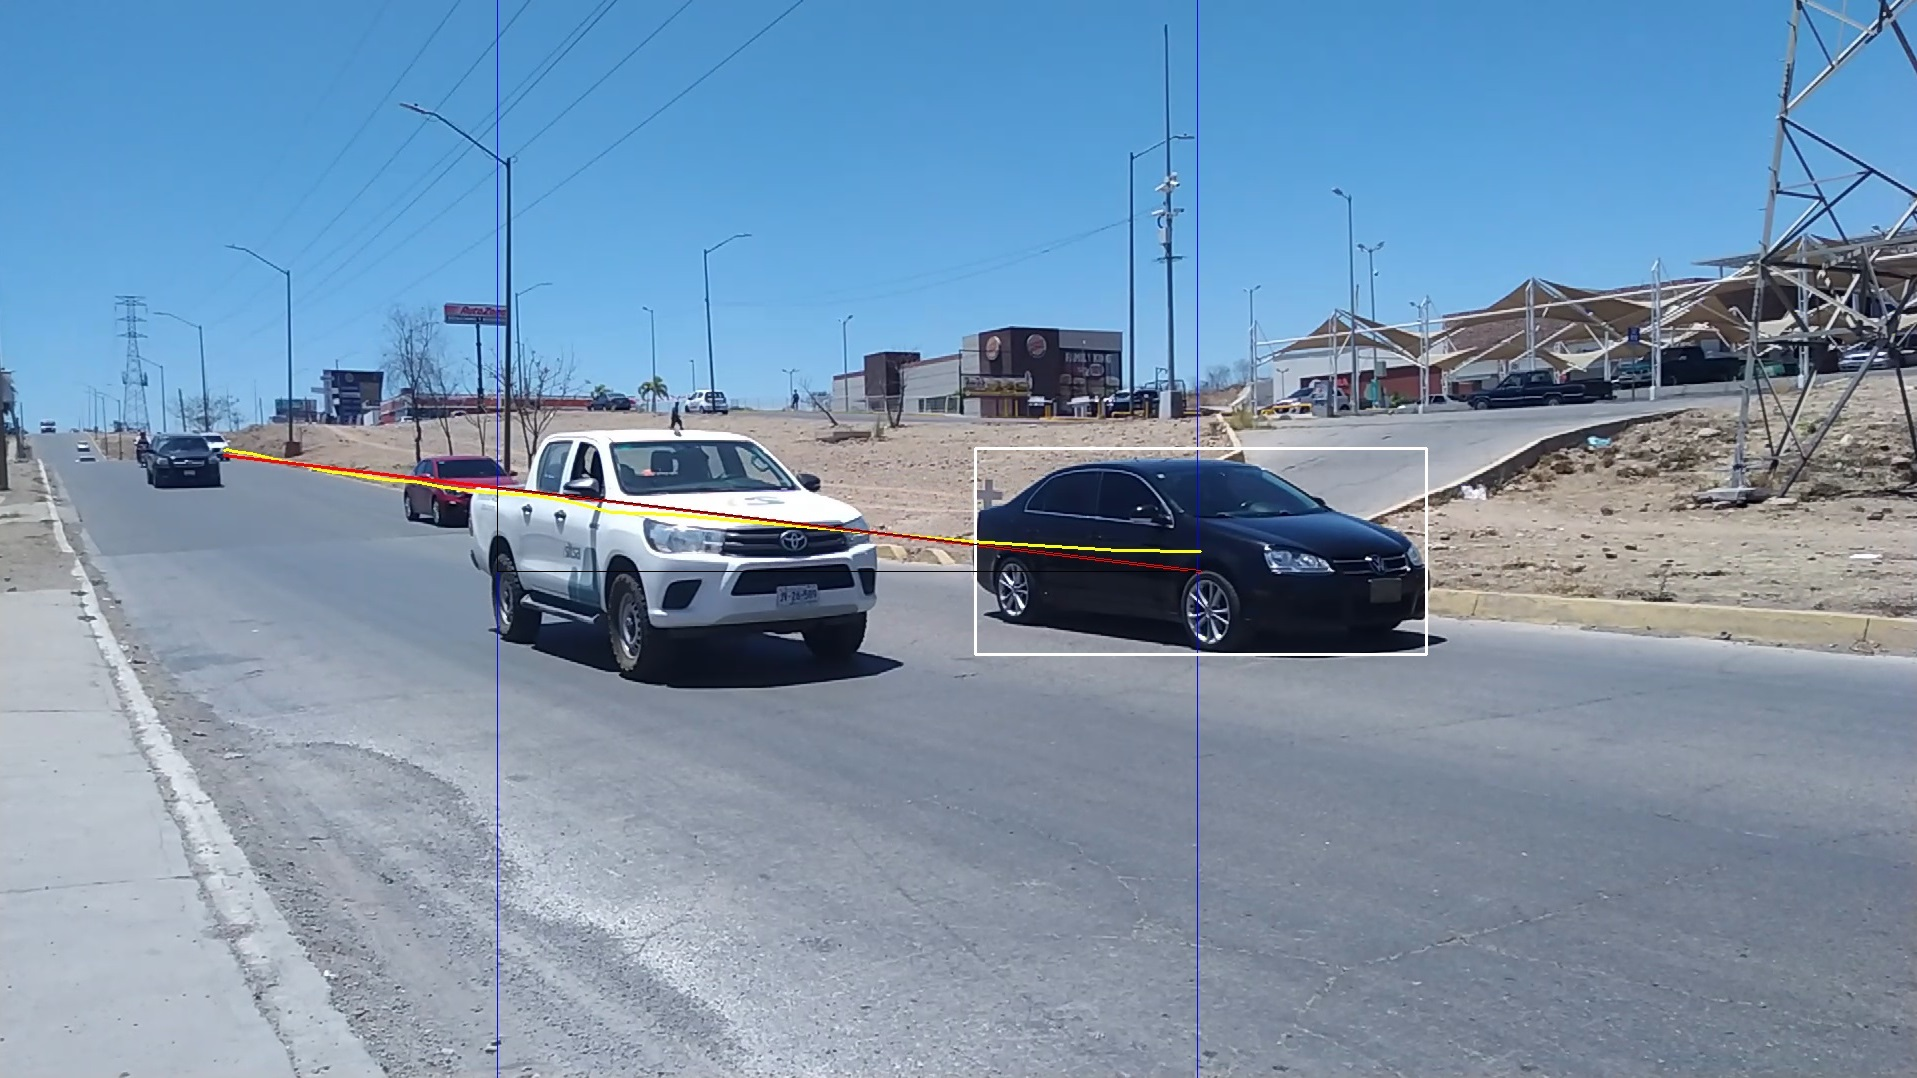
\includegraphics[width=0.8\textwidth]{Metodologia/imgs/Punto_B.jpg}
    \caption{Punto B con vehículo en recuadro blanco.}
    \label{fig:PuntoB}
\end{figure}

La Tabla \ref{tab:CaracteristicasSistema} muestra las características más importantes generadas por el sistema y su descripción.

\begin{table}[H]
    \caption{Características obtenidas por el sistema.}
    \label{tab:CaracteristicasSistema}
    \begin{tabular}{|l|l|}
        \hline
        \textbf{Característica} & \multicolumn{1}{c|}{\textbf{Descripción}} \\ \hline
        \textbf{Angulo Salida} & Angulo a partir del punto de entrada hasta el punto de salida \\ \hline
        \textbf{Distancia de salida} & Distancia recorrida desde el punto de entrada hasta el punto de salida \\ \hline
        \textbf{Área Entrada} & Área detectada del vehículo en pixeles en el punto de entrada \\ \hline
        \textbf{Área Salida} & Área detectada del vehículo en pixeles en el punto de salida \\ \hline
        \textbf{FPS} & Fotogramas por segundo del video \\ \hline
        \textbf{Tiempo} & Tiempo que le tomo al vehículo para pasar del punto entrada al de salida \\ \hline
        \textbf{Velocidad} & Velocidad detectada por el radar \\ \hline
        \textbf{Carril} & Carril por que pasa el vehículo \\ \hline
        \textbf{Identificador} & Identificador correspondiente a una imagen generada \\ \hline
    \end{tabular}
\end{table}


El sistema además de generar un archivo CSV, nos crea una imagen de salida la cual corresponde a una línea del archivo resultante, esta imagen está formada por dos imágenes una al lado de la otra, la imagen de la izquierda representa el vehículo cuando entra en el punto A y la imagen de la derecha es cuando el vehículo pasa por el punto B. La Figura \ref{fig:Completo} muestra un ejemplo de esta imagen de salida.

\begin{figure}[H]
    \centering
    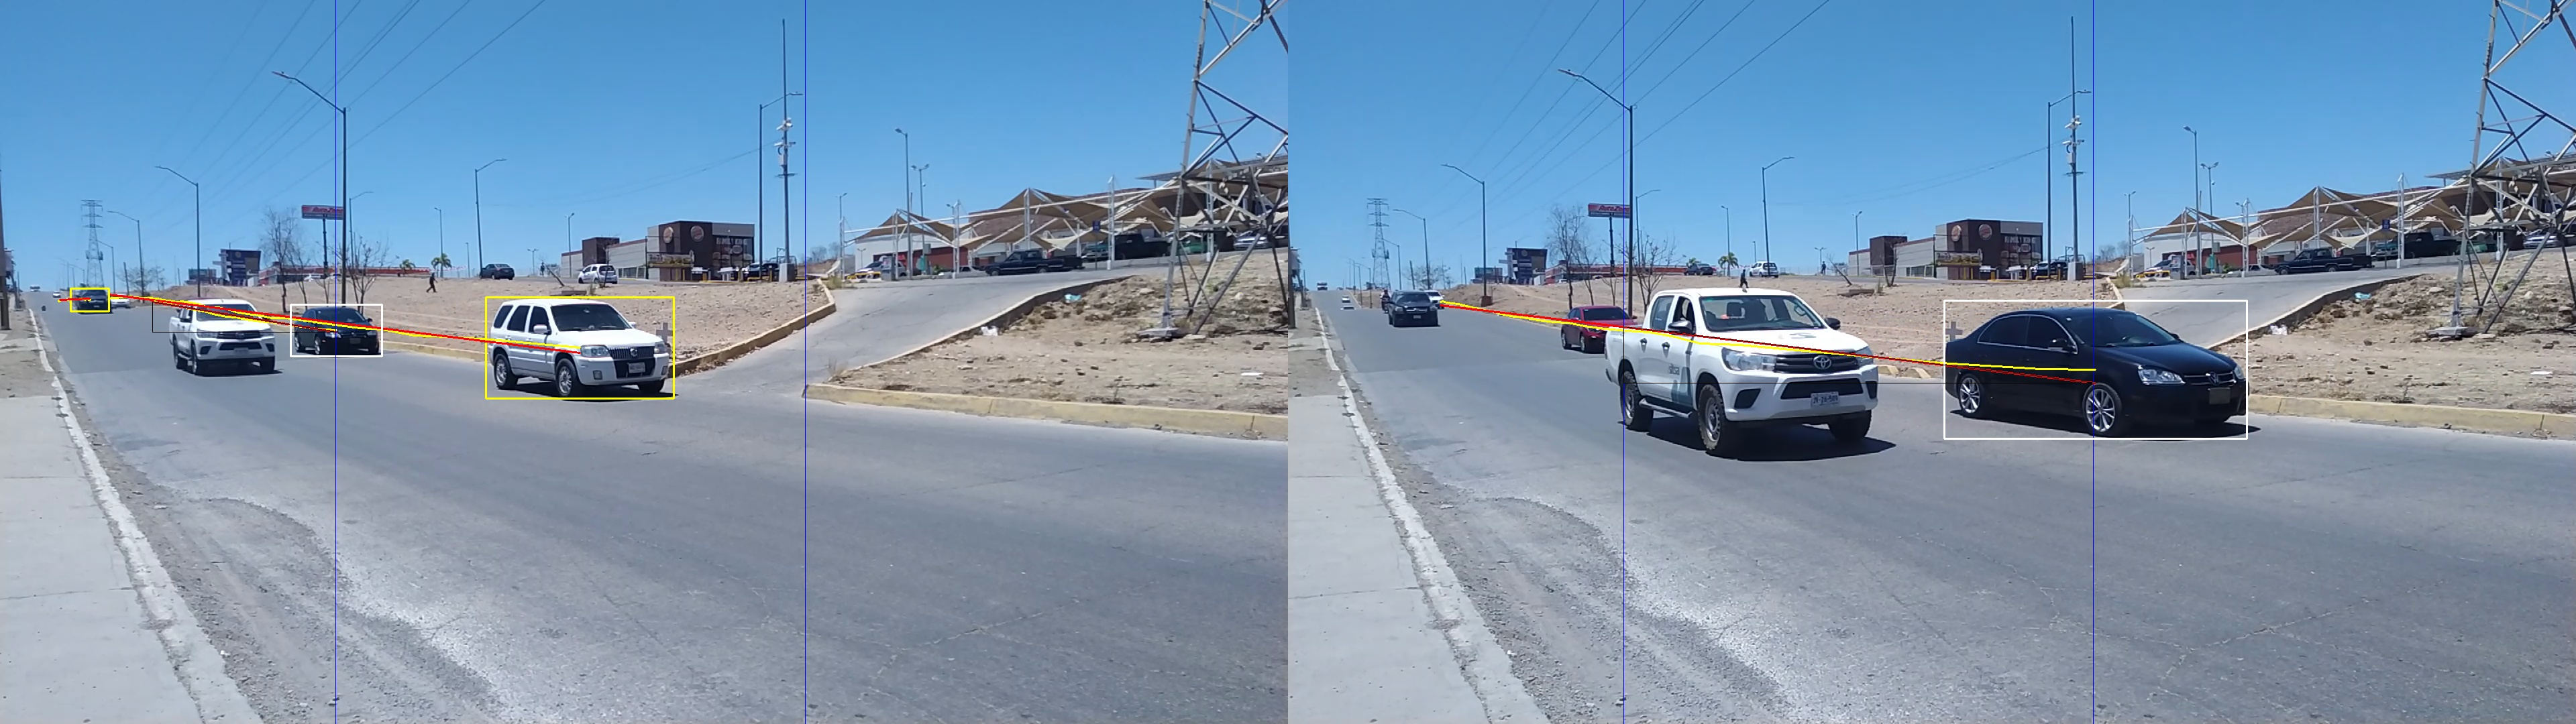
\includegraphics[width=1\textwidth]{Metodologia/imgs/Completo.jpg}
    \caption{Imagen resultado para cada linea de archivo CSV.}
    \label{fig:Completo}
\end{figure}

%%%%%%%%%%%%%%%%%%%%%%%%%%%%%%%%%%%%%%%%%%%%%%%%%%%%%%%%%%%%%%%%%%%%%%%%%%%%%%%%
%%%%%%%%%%%%%%%%%%%%%%%%%%%%%%%%%%%%%%%%%%%%%%%%%%%%%%%%%%%%%%%%%%%%%%%%%%%%%%%%
%%%%%%%%%%%%%%%%%%%%%%%%%%%%%%%%%%%%%%%%%%%%%%%%%%%%%%%%%%%%%%%%%%%%%%%%%%%%%%%%
%%%%%%%%%%%%%%%%%%%%%%%%%%%%%%%%%%%%%%%%%%%%%%%%%%%%%%%%%%%%%%%%%%%%%%%%%%%%%%%%
%%%%%%%%%%%%%%%%%%%%%%%%%%%%%%%%%%%%%%%%%%%%%%%%%%%%%%%%%%%%%%%%%%%%%%%%%%%%%%%%

Una vez que el sistema genera nuestras imágenes de salida y el archivo CSV resultante debemos validar que el vehículo detectado sea el correcto y que el área de detección del vehículo sea lo más completa posible.

Para el caso de validar que el vehículo sea el correcto debemos ver cada una de las imágenes generadas y leer la descripción en el archivo CSV de entrada, en caso de identificar un vehículo que no corresponda debemos modificar los segundos en el archivo CSV de entrada de tal manera que el sistema detecte el vehículo  correcto, existen dos casos en los que el sistema no podrá identificar el vehículo, que el vehículo correcto sea tapado por otro o que al vehículo no se le haya podido generar su seguimiento completo del punto A al B de forma correcta, para estos caso debemos eliminar la línea correspondiente en el archivo de entrada, para ambos casos ya sea que se tenga que modificar los segundos o se tenga que eliminar la línea debemos ejecutar el sistema nuevamente para que el sistema genere todo de nuevo.

Para validar que el área de detección del vehículo sea lo más completa posible también debemos realizar una inspección visual de las imágenes generadas, en estas podemos identificar cuando un vehículo ha sido detectado completamente, como muestra la Figura \ref{fig:ImagenValida}.

\begin{figure}[H]
    \centering
    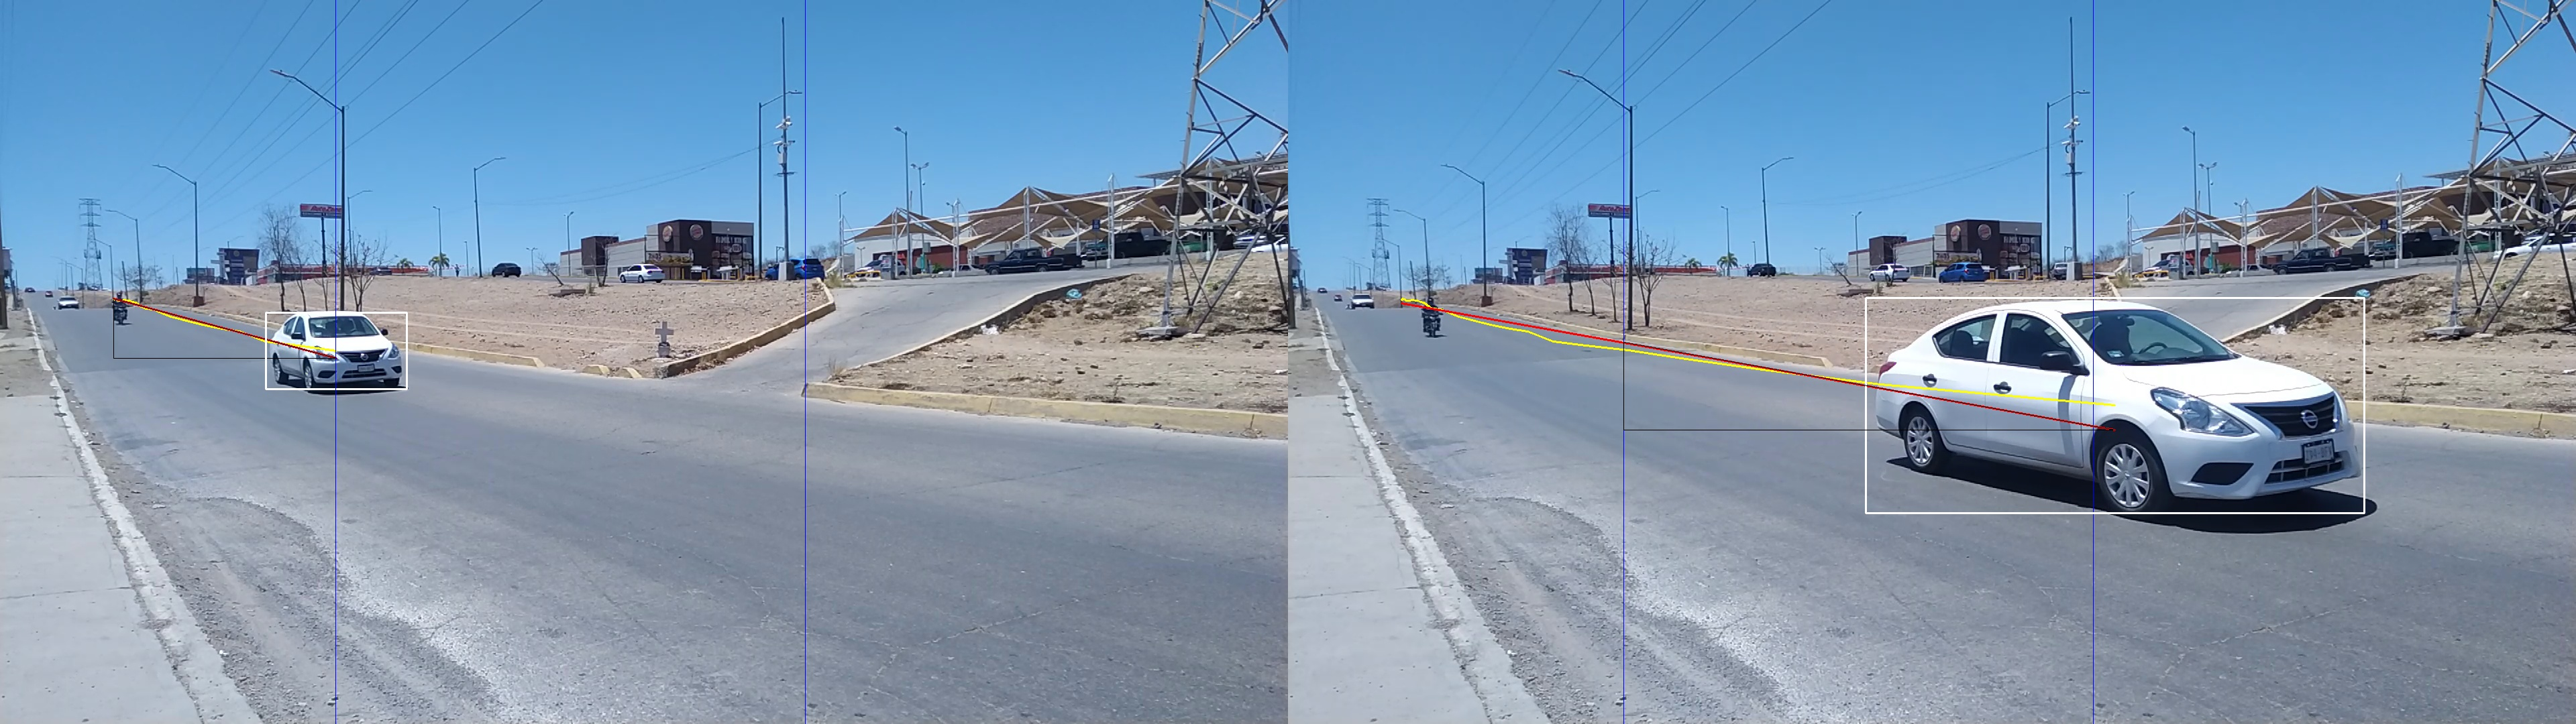
\includegraphics[width=1\textwidth]{Metodologia/imgs/Valido.jpg}
    \caption{Imagen valida representando una linea del archivo CSV.}
    \label{fig:ImagenValida}
\end{figure}

Por otra parte, hay ocasiones en la cuales el sistema solo detecta parte del vehículo, estas imágenes son las que podemos considerar como invalidas, un ejemplo se muestra en la Figura \ref{fig:ImagenInvalida}.

\begin{figure}[H]
    \centering
    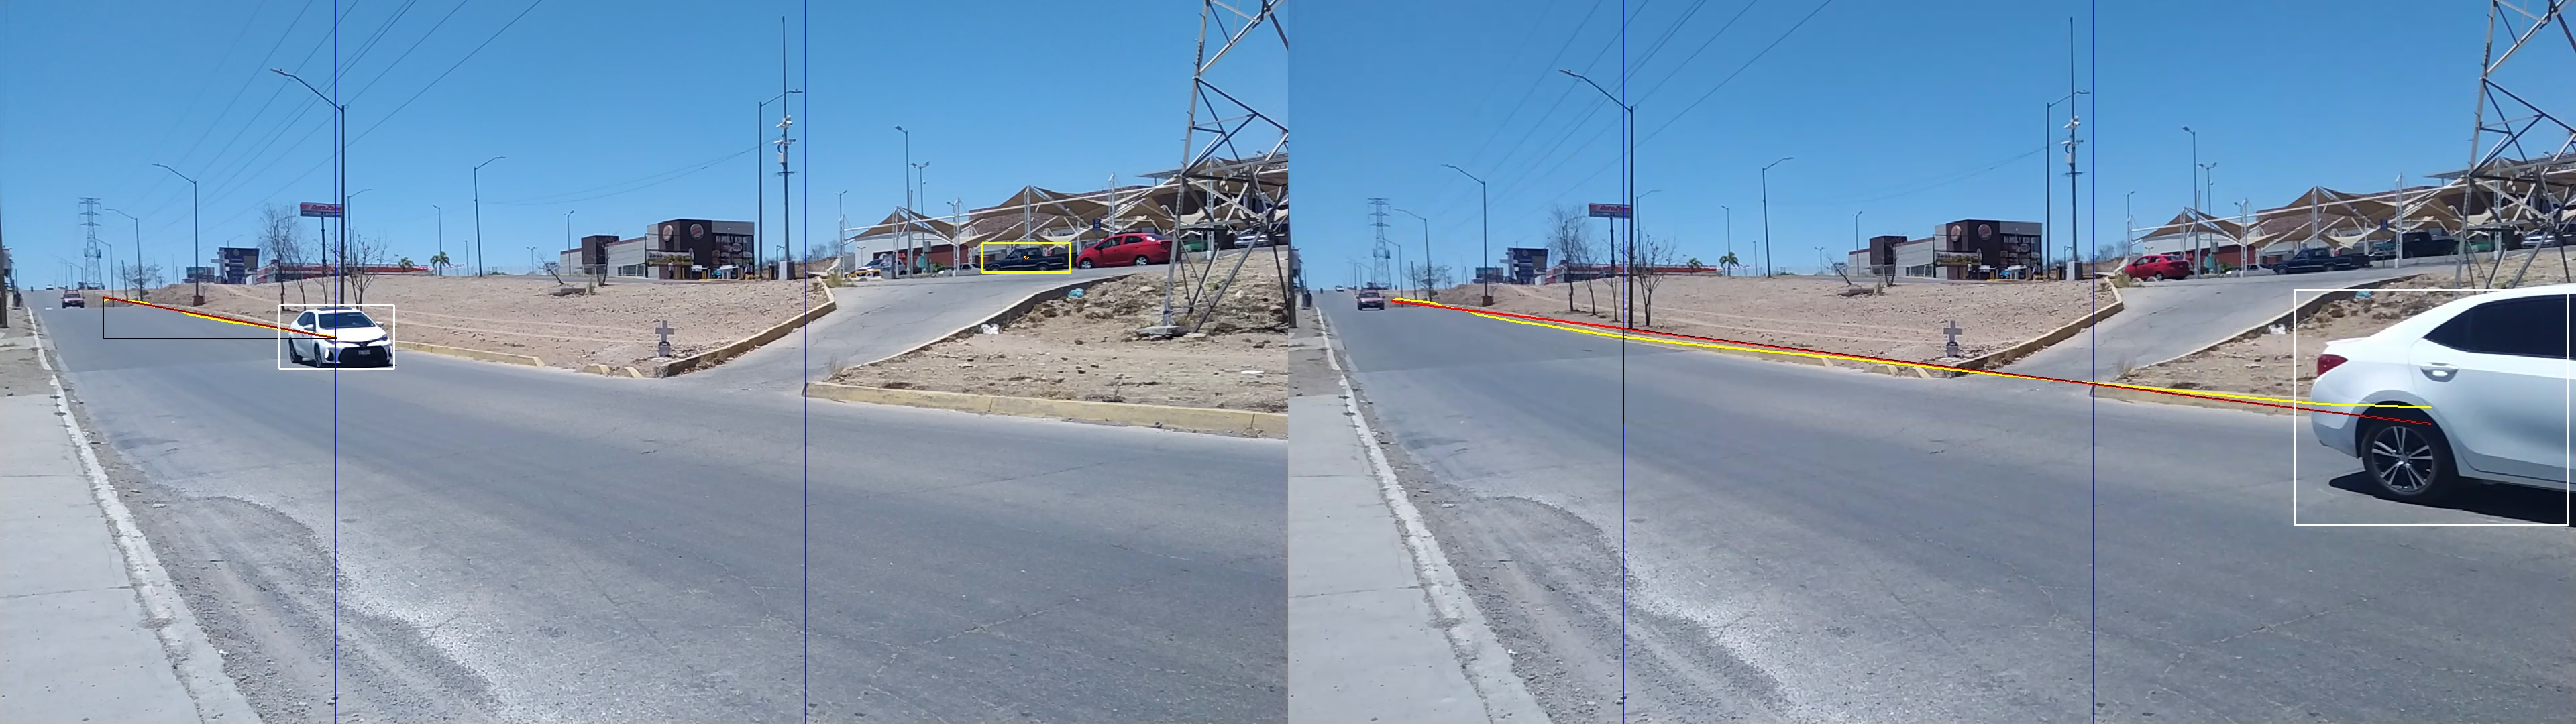
\includegraphics[width=1\textwidth]{Metodologia/imgs/Invalido.jpg}
    \caption{Imagen invalida representando una linea del archivo CSV.}
    \label{fig:ImagenInvalida}
\end{figure}

Una vez que encontramos una imagen invalida procedemos a eliminar la línea correspondiente en el archivo CSV de salida, esta línea la podemos identificar por el identificador del final ya que este corresponde a la imagen. Para este caso no es necesario volver a ejecutar el sistema, pero se recomienda hacer un respaldo del archivo CSV original para futuras referencias.

